\documentclass[12pt]{article}

\usepackage[longnamesfirst]{natbib}
\usepackage{amssymb}
\usepackage{amsmath}
\usepackage{bm}
\usepackage{dsfont}
\usepackage[margin=1.25in]{geometry}
\usepackage[font=scriptsize]{caption}
\usepackage{dsfont}
\usepackage{amsmath}
\usepackage{graphicx}
\usepackage{bm}
\usepackage{float}
\newcommand{\m}[1]{\mathbf{\bm{#1}}}
\newcommand{\R}{I\hspace{-4.4pt}R}
\newcommand{\bc}[1]{\textcolor{blue}{\mathbf{#1}}}
\newcommand{\ind}{\mathds{1}}
% \newcommand{\symsquare}{\begin{tiny}$\blacksquare$\end{tiny}}
% \newcommand{\symcircle}{\begin{footnotesize}$\bullet$\end{footnotesize}}
% \newcommand{\symtriangle}{\begin{scriptsize}$\blacktriangle$\end{scriptsize}}

\newcommand{\symsquare}{{\tiny $\blacksquare$}}
\newcommand{\symcircle}{{\footnotesize $\bullet$}}
\newcommand{\symtriangle}{{\scriptsize $\blacktriangle$}}


% \setlength\parindent{0pt}

\begin{document}

\begin{Large}
\noindent \textbf{Hierarchical estimation of the extremal index}
\end{Large}
\bigskip

%\begin{large}
\noindent \textbf{Mickey Warner}
%end{large}

\section{Abstract}
\label{abstract}

This paper extends estimation of the extremal index to the hierarchical setting based on likelihoods provided by \cite{ferro2003inference} and \cite{suveges2010model}.            The hierarchical model is applied to simulated data and with CanCM4 climate model simulations.


\section{Introduction}
\label{intro}

In extreme value analysis, a primary interest is in modeling the upper tail of a sequence of random variables $X_1,\ldots,X_n$ each with marginal distribution $F$. The standard approach begins by selecting a threshold $u$ and assuming the exceedances $Y_i=X_i-u$ follow a generalized Pareto distribution having distribution function
\[ H(y) = 1 - \left(1 + \xi \frac{y}{\sigma}\right)^{-1/\xi} \]
for $y>0$ defined on $\{y:1+\xi y/\sigma>0\}$. The assumption is based on an approximation due to asymptotic theory for which at least two conditions must be satisfied: (1) the threshold $u$ is high enough, and (2) the $X_i$'s are independent.

When the second condition is not met (which is often the case in a time-series), inference can instead be based on clusters of exceedances. That is, because of dependence between observations, it could be expected that exceedances will arrive together in groups or clusters. Clusters can be formed by choosing a run parameter $K$ and then grouping those exceedances which are seperated by no more than $K$ non-exceedances. This is called runs declustering with the clusters assumed to be independent. \cite{ferro2003inference} provide a method for automatically declustering observations based on an estimate of the extremal index.

The extremal index, $\theta$, appears in the following way (see \cite{coles2001introduction}). For stationary process $X_1,X_2,\ldots$ with marginal distributions $F$, and $X_1^*,X_2^*,\ldots$ independent with marginal distributions $F$, let $M_n=\max(X_1,\ldots,X_n)$, and $M_n^*=\max(X_1^*,\ldots,X_n^*)$. Under suitable regularity conditions
\[ P((M_n-b_n)/a_n \leq z) \rightarrow G_1(z) \]
as $n\rightarrow\infty$ for normalizing sequences $a_n>0$ and $b_n$, where $G_1$ is a non-degenerate distribution function, if and only if
\[ P((M_n^*-b_n)/a_n \leq z) \rightarrow G_2(z),\]
where
\[ G_2(z)=G_1^\theta(z) \]
for $\theta\in(0,1]$. The extremal index plays the important role of controlling the cluster size of exceedances by the following, loose, interpretion
\[ \theta = (\mathrm{limiting~mean~cluster~size})^{-1}. \]
Therefore, if $\theta$ is known, we can form clusters such that our average cluster size is roughly $\theta^{-1}$.

Our interest in this paper is to extend the estimators of $\theta$ provided by \cite{ferro2003inference} and \cite{suveges2010model} to a hierarchical setting. In a time-series analysis, it is uncommon, and sometimes impossible, to have multiple realizations of a stochastic process over the same time domain. For example, we cannot go back in time, tweak a few variables, and observe new climatological data. With a computer model, there is no such constraint. Even for a deterministic model, variability can be induced by evaluating the model at a variety of input settings. Hence, we have several time-series that have their own extremal index, but it is believed that there is a commonality between them. The hierarchical model will also allow us to make inference on a climate simulation not yet observed.

Estimation of the extremal index is based on the asymptotic distribution of interarrival times. Suppose we have observations $X_1,\ldots,X_n$. For a threshold $u$, the $N$ exceedances $Y_i=X_i-u$ given $X_i>u$ occur at times $1\leq j_1<\cdots< j_N\leq n$. The observed interexceedance times are given by $T_i=j_{i+1}-j_i$ for $i=1,\ldots,N-1$.

\cite{ferro2003inference} produce the following log-likelihood for $\theta$
\begin{align}
l_1(\theta, p; \m{T}) =& m_1\log(1-\theta p^\theta) + (N-1-m_1)\{\log(\theta)+ \log(1-p^\theta)\} \nonumber \\
 &+ \theta\log(p)\sum_{i=1}^{N-1}(T_i-1) \label{ferro}
\end{align}
where $m_1=\sum_{i=1}^{N-1}\ind(T_i=1)$ and $p=F(u)=1-\overline{F}(u)$. \cite{suveges2010model} defines $S_i^{(K)}=\max\{T_i-K,0\}$ and gives this log-likelihood
%\[ L_2(\theta, p)= (1-\theta)^{N-1-N_C}\theta^{2N_C}e^{-\theta (1-p) \sum_{i=1}^{N-1}S_i}. \]
\begin{align}
l_2(\theta, p; \m{S}^{(K)})= (N-1-N_C)\log(1-\theta)+2N_C\log(\theta)-\theta (1-p) \sum_{i=1}^{N-1}S_i^{(K)}. \label{suveges}
\end{align}
where $N_C=\sum_{i=1}^{N-1}\ind(S_i^{(K)} \neq 0)$. 


\section{Hierarchical model}
\label{model}

Suppose we have $R$ simulations from a climate model. If we assume these simulations are indepedent from each other, then we expect there to be $R$ unique extremal indices $\theta_1,\ldots,\theta_R$. However, since these all come from the same climate model, we may wish to assume that the $\theta_i$ come from a common distribution
\[ \theta_i \overset{iid}\sim Beta\left(\theta\nu, (1-\theta)\nu\right). \]
Under model (\ref{ferro}), we place a similar prior on the $p_i$
\[ p_i \overset{iid}\sim Beta\left(p\tau, (1-p)\tau\right). \]
Since model (\ref{suveges}) does not properly allow for the estimation of $p_i$, we fix each $p_i$ to be the empirical estimate of $F_i(u)$.

The model is completed by choosing priors for $\theta$, $\nu$, $p$, and $\tau$---the latter two parameters being required only for model (\ref{ferro}). We assume
\begin{align*}
\theta &\sim Beta(a_\theta, b_\theta) \\
\nu &\sim Gamma(a_\nu, b_\nu) \\
p &\sim Beta(a_p, b_p) \\
\tau &\sim Gamma(a_\tau, b_\tau) 
\end{align*}
with the hyperparameters assumed to be
%\begin{table}[h]
\begin{center}
\begin{tabular}{rlcl}
$\theta$: & $a_\theta = 1/2        $ &~~& $b_\theta = 1               $ \\
$   \nu$: & $   a_\nu = 1          $ &~~& $   b_\nu = 1/10            $ \\
$     p$: & $     a_p = 100 \hat{F}$ &~~& $     b_p = 100 (1-\hat{F}) $ \\
$  \tau$: & $  a_\tau = 1          $ &~~& $  b_\tau = 1/10            $ \\
\end{tabular}
\end{center}
%\end{table}


\section{Simulation study}
\label{sim}

We apply the hierarchical model to simulations from a max-autoregressive process. Choose $\theta_i\in(0,1]$ for $i=1,\ldots,R$. Let $W_{i,1}\ldots,W_{i,n}$ be independent unit Fr{\'e}chet random variables, and define
\begin{align}
Y_{i,1} &= W_{i,1}/\theta_i \nonumber \\
Y_{i,j} &= \max\{(1-\theta_i)Y_{i,j-1}, W_{i,j}\}~~~~~j=2,\ldots,n \label{max}
\end{align}
then $Y_{i,\cdot}$ is stochastic process having extremal index $\theta_i$. We let $R=10$, $n=1000$, and $\theta_1=\cdots=\theta_R$.

Comparisons between models (\ref{ferro}) and (\ref{suveges}) are made using coverage and RMSE.

% \begin{figure}
% 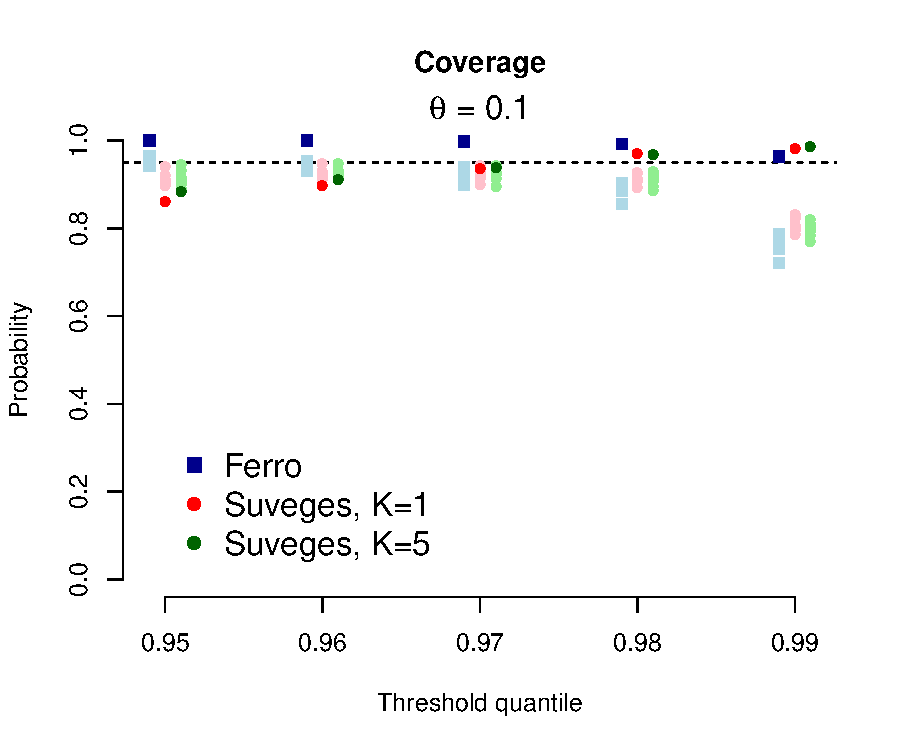
\includegraphics[scale=0.49]{../extremal_comparison/figs/sim_coverage_10.pdf}
% 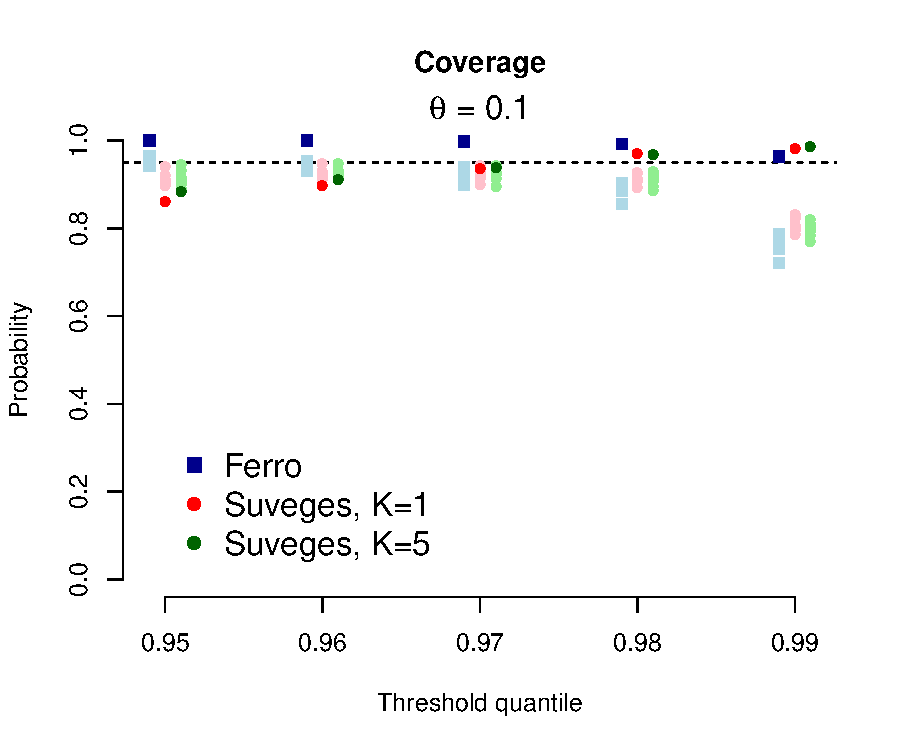
\includegraphics[scale=0.49]{../extremal_comparison/figs/sim_coverage_10.pdf}
% 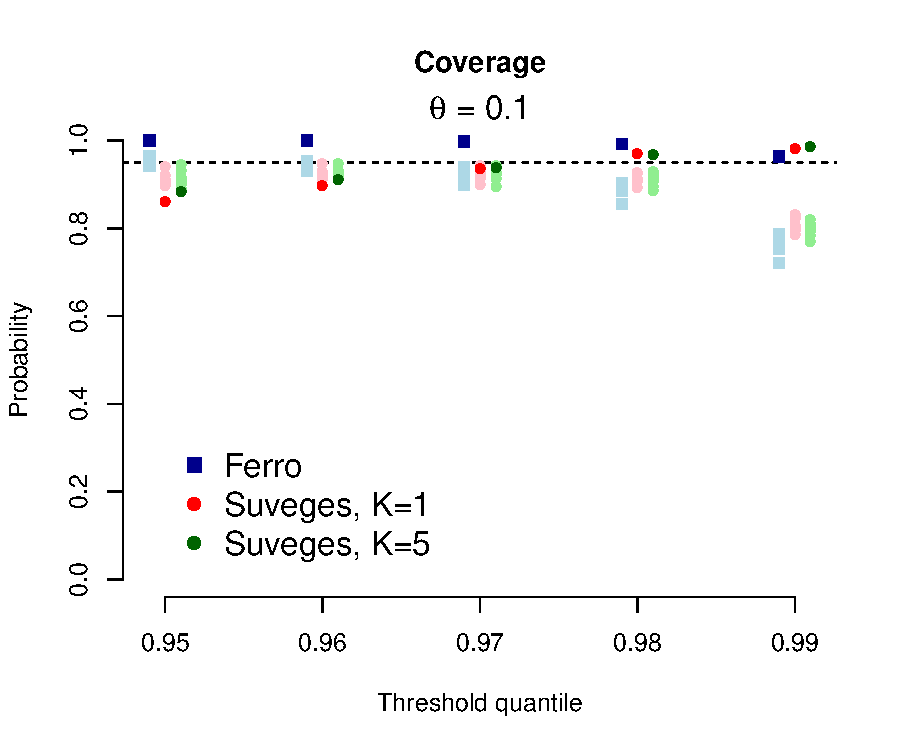
\includegraphics[scale=0.49]{../extremal_comparison/figs/sim_coverage_10.pdf}
% \end{figure}
% 
% \begin{figure}
% 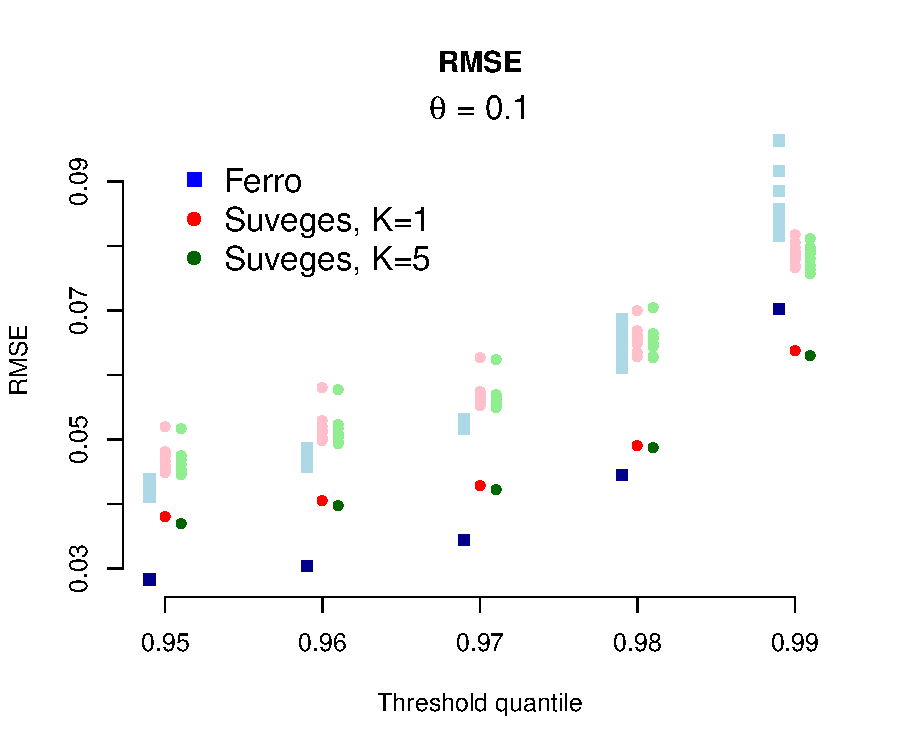
\includegraphics[scale=0.3]{../extremal_comparison/figs/sim_rmse_10.pdf}
% 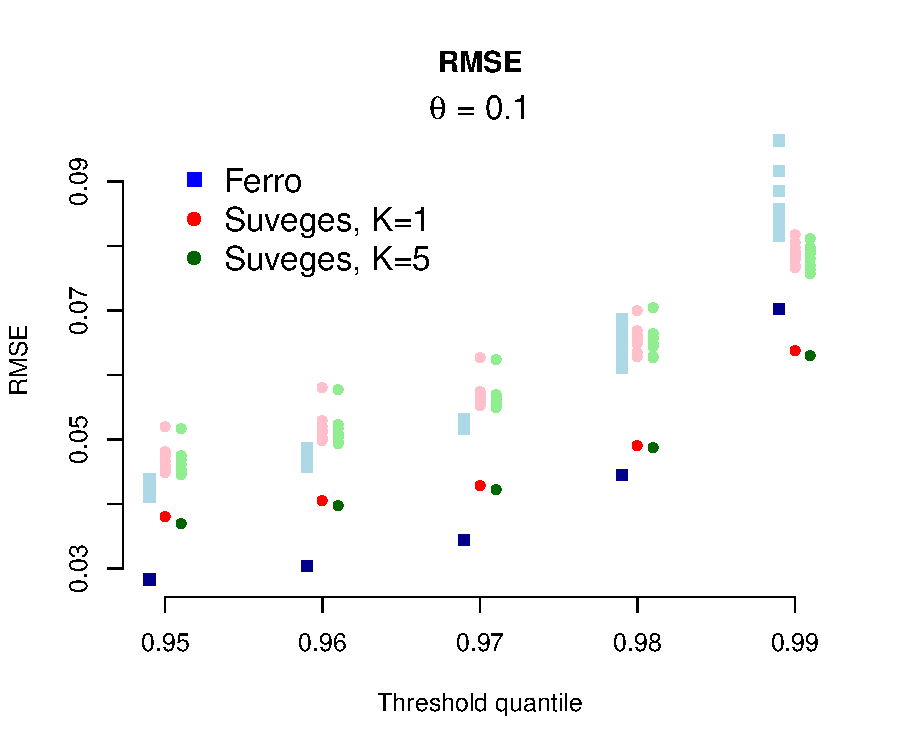
\includegraphics[scale=0.3]{../extremal_comparison/figs/sim_rmse_10.pdf}
% 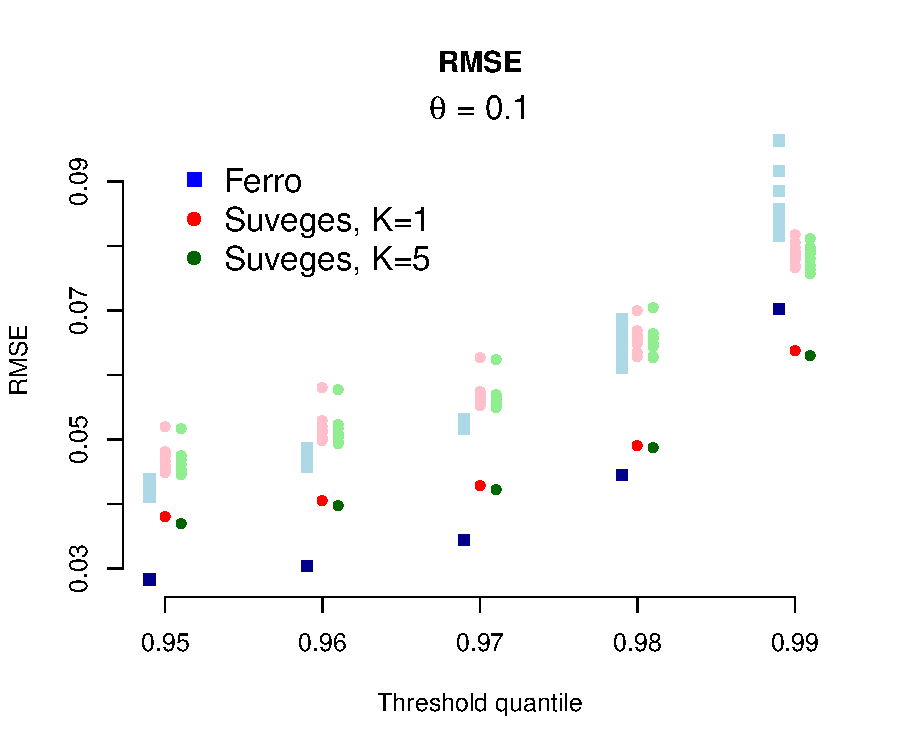
\includegraphics[scale=0.3]{../extremal_comparison/figs/sim_rmse_10.pdf}
% \end{figure}

\begin{figure}
\begin{center}
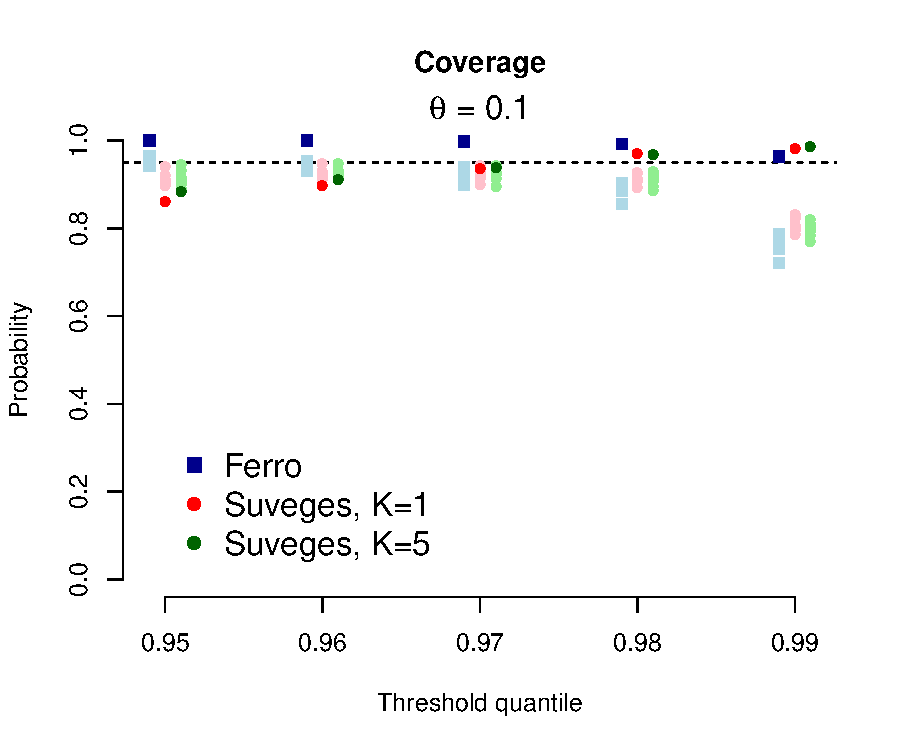
\includegraphics[scale=0.48]{../extremal_comparison/figs/sim_coverage_10.pdf}
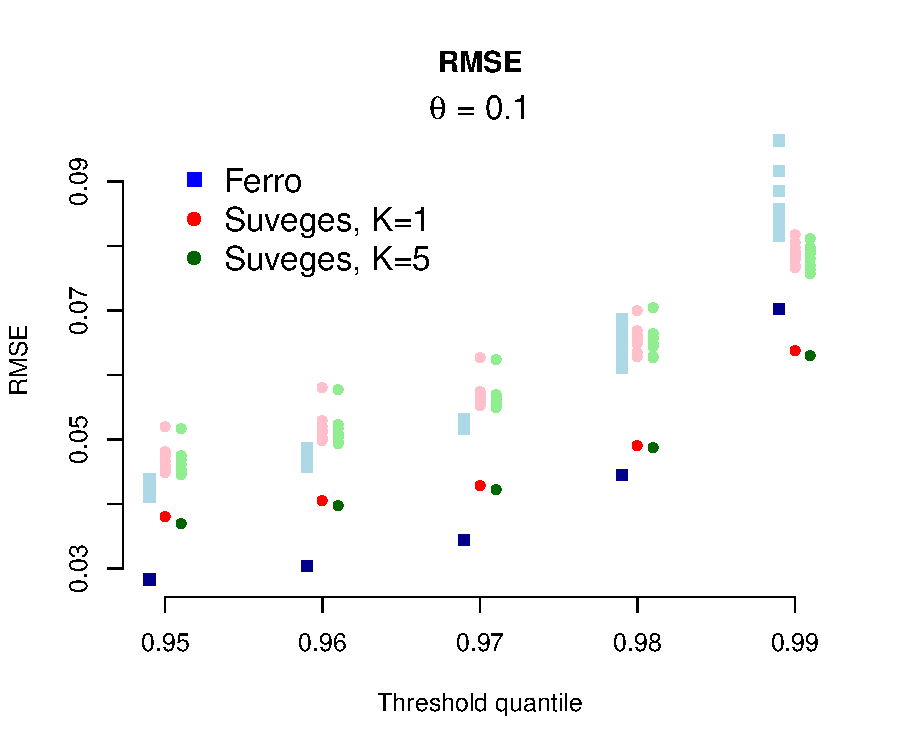
\includegraphics[scale=0.48]{../extremal_comparison/figs/sim_rmse_10.pdf}
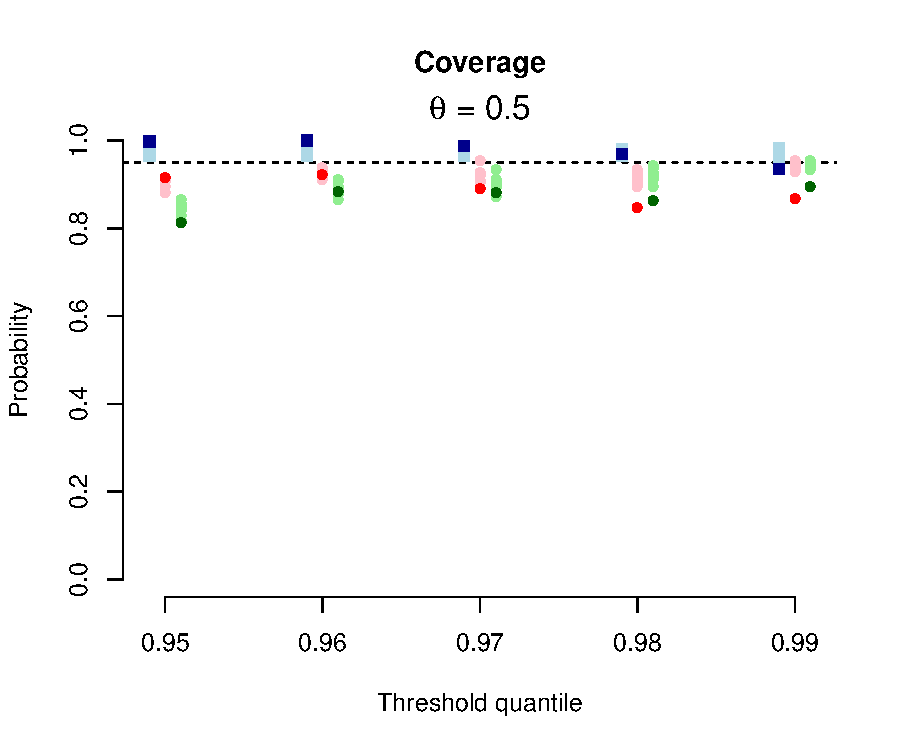
\includegraphics[scale=0.48]{../extremal_comparison/figs/sim_coverage_50.pdf}
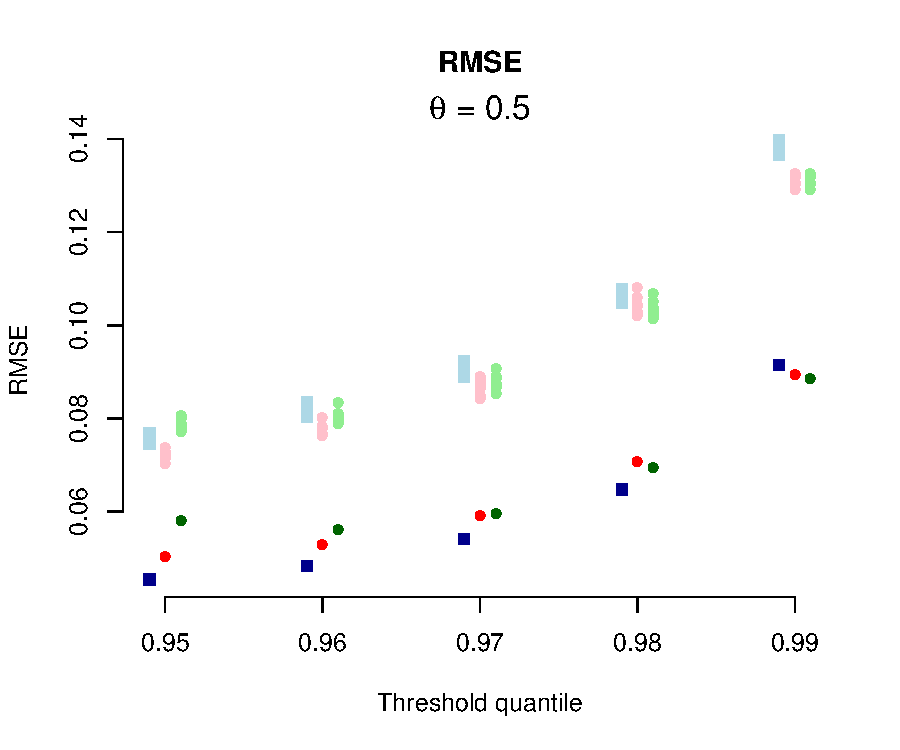
\includegraphics[scale=0.48]{../extremal_comparison/figs/sim_rmse_50.pdf}
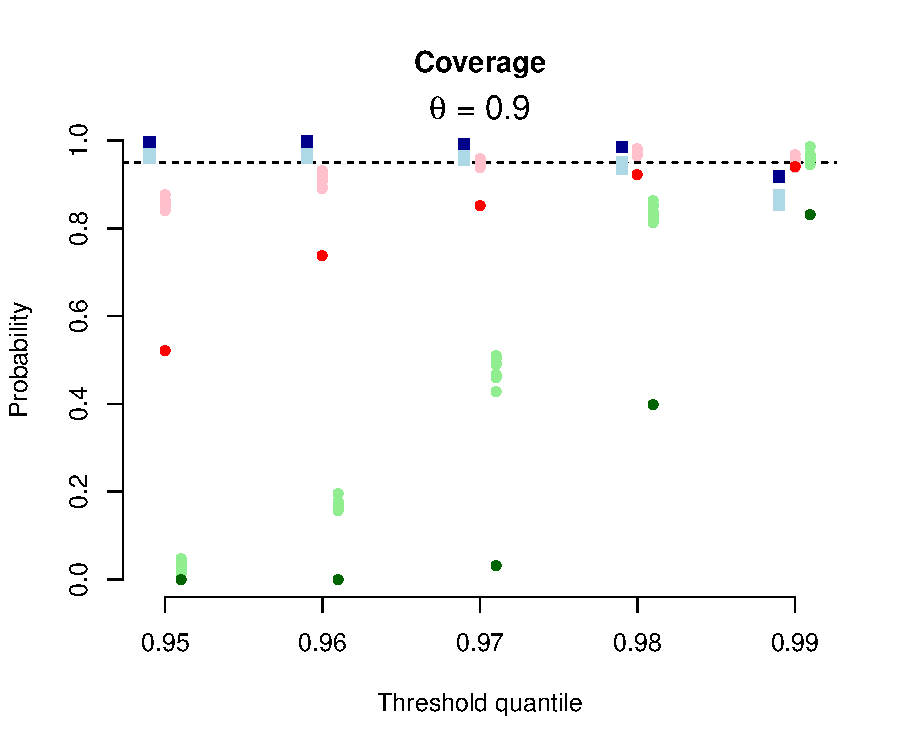
\includegraphics[scale=0.48]{../extremal_comparison/figs/sim_coverage_90.pdf}
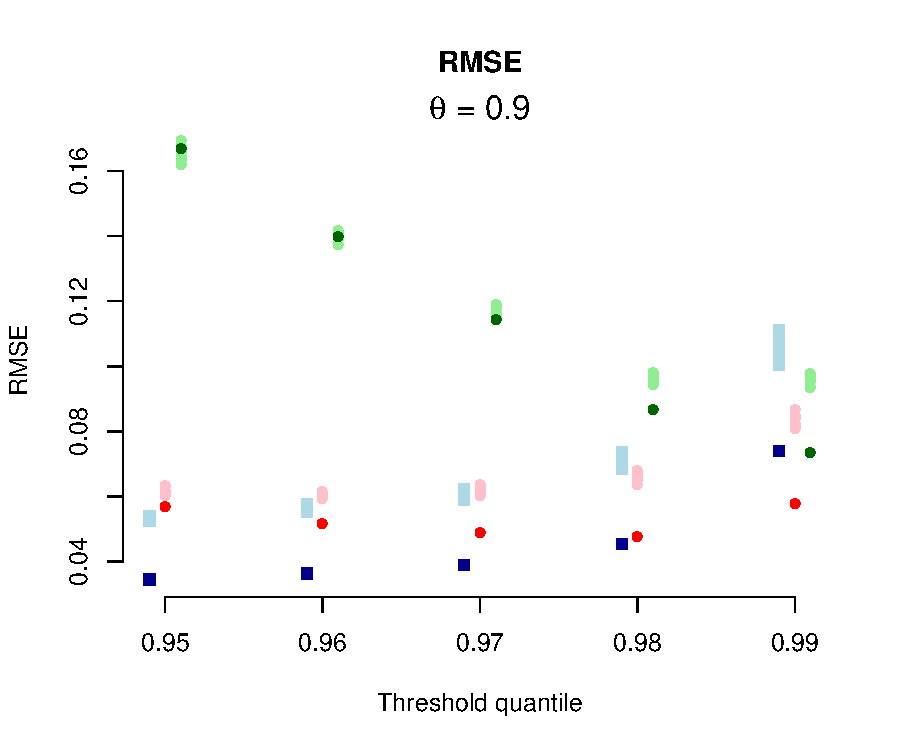
\includegraphics[scale=0.48]{../extremal_comparison/figs/sim_rmse_90.pdf}
\end{center}
\caption{Coverage (left column) and RMSE (right) for the two likelihoods in the simulation study. Each row is based on a different extremal index, either $0.10$, $0.50$, or $0.90$. The darker points represent the hierarchical mean, the lighter points are from the individual sequences. The nominal coverage probability (0.95) is marked by the dashed horizontal line.}
\label{simfigs}
\end{figure}


\section{Climate model simulations}
\label{climate}

The Fourth Generation Coupled Global Climate Model (called CanCM4, here) produces a wide array of atmospheric conditions across the globe. Three experimental settings that are of particular interest are decadal, historical, and pre-industrial control runs. (Description of the type of simulations).

Decadal and historical simulations are run at $R=10$ different input settings. To obtain $R=10$ ``replicates'' for the control simulations, we randomly select ten non-overlapping 10-year periods. Our assumption is that each replicate is independent and has related extremal indexes within their respective simulation class.

We will look at daily winter precipitation and summer maximum temperature, both over California during the 1990s. The quantities used in the analysis are total precipitation (a weighted sum) and average maximum temperature (weighted). (EXPAND). This leads to a $R$ univariate time series for each class of simulations. To each time-series is fit a dynamic linear model (DLM) having the first two harmonics. Anomalies are computed by taking the difference of the time-series and the smoothed predictions based on the DLM. For winter we look at only December, January, and February. For summer we have June, July, and August. Finally, we treat the time-series as though there is no gap between the seasons of interest. For example, 28 February is followed immediately by 1 December in the winter analysis. This completes our pre-processing. (After the processing, the sequences are assumed stationary).

A comparison of each simulation class and likelihood is found in Figures \ref{figwinter} and \ref{figsummer}. (Not $K=5$ yet). In every situation we see that the estimates for $\theta$ are increasing with threshold (Check: Is this happening in the simulation study?). For a given likelihood, the means for the extremal index in each simulation class are roughly the same. We do not observe this for a given class: there is clearly a discrepancy between the estimates provided by the two likelihoods. However, in all cases, the 95\% probability intervals more or less overlap.

\begin{figure}
\begin{center}
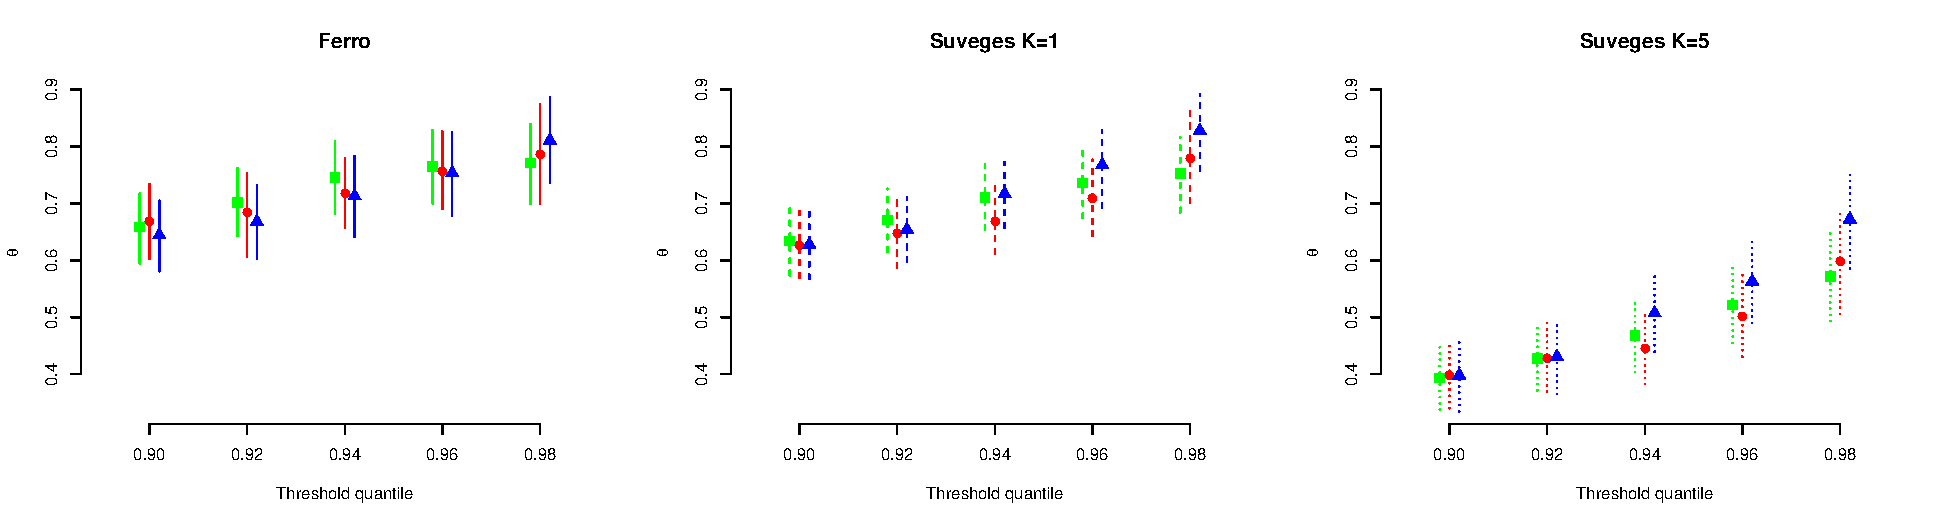
\includegraphics[scale=0.46]{figs/winter_like.pdf}
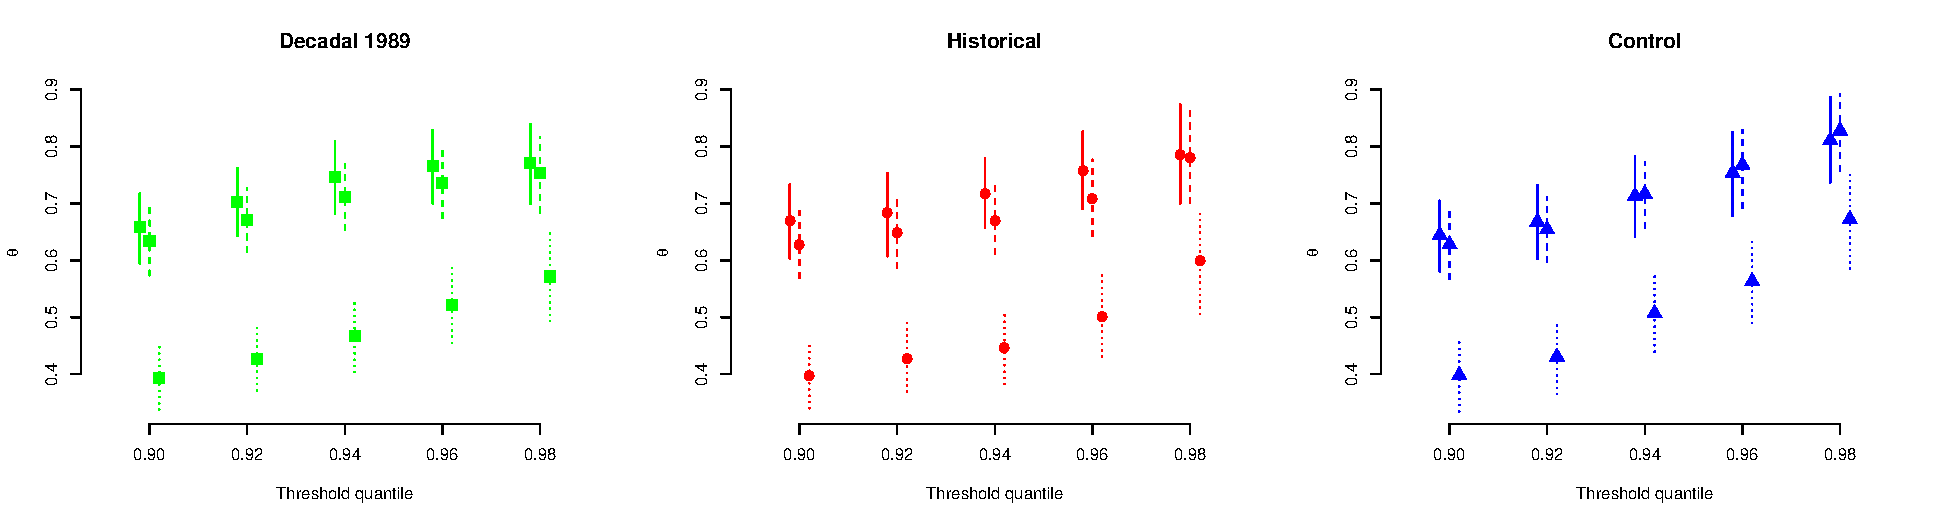
\includegraphics[scale=0.46]{figs/winter_source.pdf}
\end{center}
\caption{Both rows show the same information, but are arranged differently. The top row compares the extremal indexes of the climate models for a given likelihood. The bottom row compares the two likelihoods for each climate model. Solid lines (-----) denote model M1, dashed lines (- - -) denote M2 and dotted lines ($\cdot\cdot\cdot$) denote M3. Squares (\symsquare) mark decadal runs, dots (\symcircle) mark historical runs, and triangles (\symtriangle) are control runs. The points are the posterior means and the lines are 95\% h.p.d. intervals. The domain is California winter precipitation from 1990--1999.}
\label{figwinter}
\end{figure}

\begin{figure}
\begin{center}
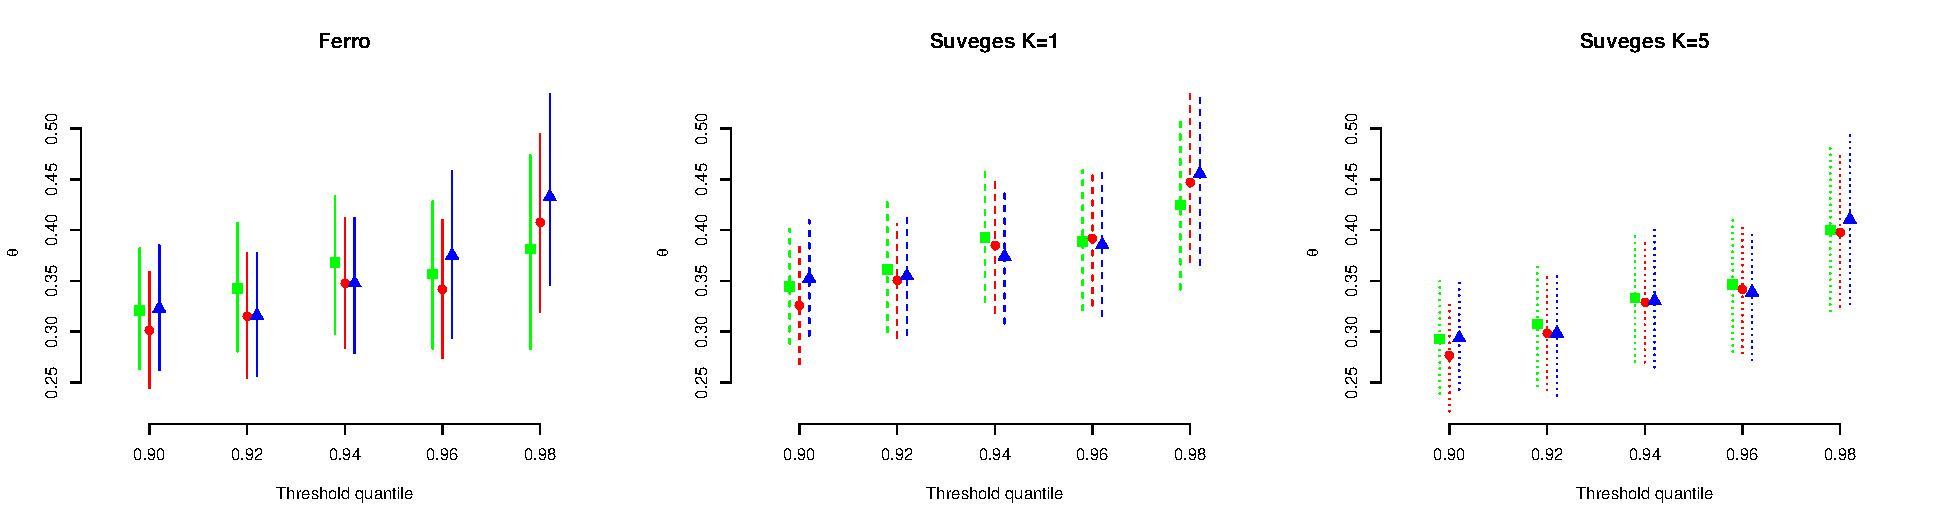
\includegraphics[scale=0.46]{figs/summer_like.pdf}
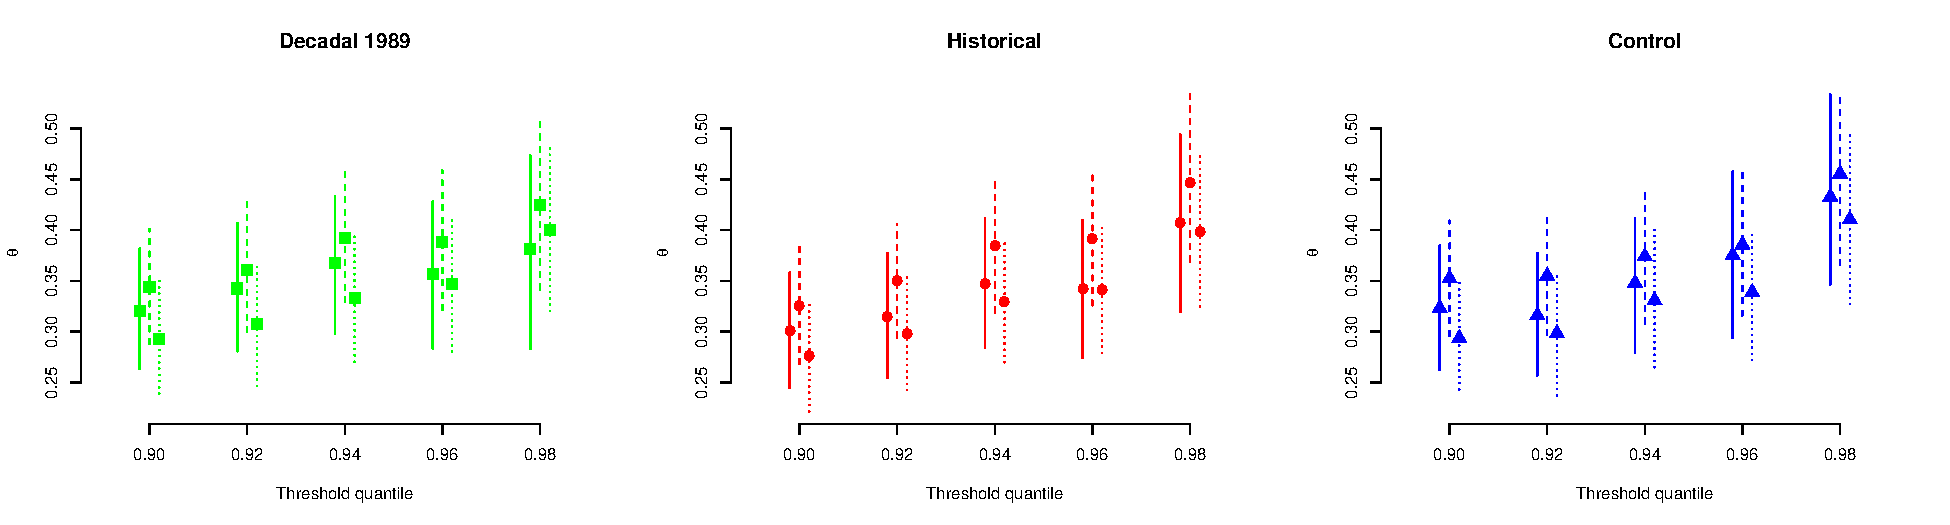
\includegraphics[scale=0.46]{figs/summer_source.pdf}
\end{center}
\caption{Same as in Figure \ref{figwinter}, but the hierarchical model is applied to summer maximum temperature.}
\label{figsummer}
\end{figure}

Where there is no overlap in intervals (see control runs for winter precipitation), we should consider how much of an issue this may be. Since the extremal index can be described as the reciprocal mean cluster size in the limit, there is a small practical difference between $0.63^{-1}=1.58$ and $0.83^{-1}=1.20$ when choosing to decluster the exceedances. The difference may be more pronounced when return levels are calculated. As $\theta$ decreases, non-overlapping posterior intervals become be much more concerning.


\section{Conclusion}
\label{conclusion}

The simulation study seems to favor the intervals estimator (\ref{ferro}) over the maximum likelihood estimator of \cite{suveges2010model} for lower thresholds. This is problematic for the obvious reasons surrounding too-low thresholds. But when working with small amounts of data, a lower threshold may be the only viable option.

Analysis of the CanCM4 simulations showed differences between the likelihoods in the estimates of the extremal index. There is also a trend for $\theta$ to increase with threshold. This could suggest at least two things. First, that we need to pick a threshold sufficiently high before convergence to the true extremal index. Second, and possibly worse, that we are seeing the issues described in \cite{ferro2003inference} regarding model (\ref{ferro}).



\bibliography{refs}
\bibliographystyle{asa}


\end{document}
